\scanpage{122}
\mspage{121}


corps et si on se borne aux modules de type fini sur $k$, on est dans les conditions de 6), et on trouve le groupe algébrique $\underline{G}_m$ sur $k$. D'ailleurs même sans condition sur $k$ et sans se borner à des modules de type fini, on récupère $C$ avec toutes ces structures par les représentations de $\underline{G}_m$\handwritten{\unsure{!|/}}

Gardons $\unsure{\otimes|\Omega}$, $\handwritten{\phi}$ (et $\underline{1},u,v$) comme dessus, mais changeons $\handwritten{\unsure{\psi|\mu}}$ \deleted{en \rlap{\unsure{l}}$\handwritten{\unsure{\phi|\psi}}$e}, en \deleted{tui} utilisant la règle de Koszul. Ce\inserted{\handwritten{nouveau}\handwritten{\begin{tikzpicture}[x=.45cm,y=.45cm,baseline=-.2ex]\draw (0,-.32) .. controls (.05,-.04) and (.16,.06) .. (.38,.08)--(1.8,.06) .. controls (2.02,.08) and (2.14,.22) .. (2.16,.45);\end{tikzpicture}}} choix de $\handwritten{\unsure{\mu|\psi}}$ s'impose dans certaines questions. Par exemple supposons $k$ un corps, \deleted{de car. nulle,} soit $V$ la catégorie des espaces topologiques compacts, avec le foncteur $\otimes$ donné pa\unsure{r} produit cartésien, et la donnée évidente d'associativité et de commutativité (pour le c\deleted{a}oup on n'a vraiment pas le choix !); il y a\deleted{\unsure{u|n}} une unité, \unsure{à} \unsure{\rlap{a}s|$\mathbb{s}$}\unsure{\rlap{s}a|$\mathbb{a}$}voir l\deleted{es}'espace\deleted{s} ponctuel. Considérons le foncteur cohomologique $X\handwritten{\mapsto}H^{\handwritten{\bullet}}(X,k)$ sur $V^{\unsure{o|0}}$, utilisant Künneth on trouve un isomorphisme $c$ de compatibilité aux $\otimes$\inserted{de $V^o$ dans $C$\handwritten{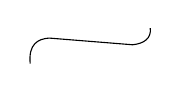
\begin{tikzpicture}[x=.5cm,y=.5cm,baseline=-.2ex]\draw (0,-.45) .. controls (-.05,.05) and (.2,.18) .. (.48,.2)--(2.6,.03) .. controls (2.9,.06) and (3.08,.2) .. (3.05,.45);\end{tikzpicture}}}. Ce dernier est compatible aux structures a),b),c) \uline{à condition} de choisir $\handwritten{\mu}$ dans $C$ par la règle de Koko\rlap{\raisebox{.65ex}{\deleted{\unsure{f}}}}\handwritten{!}

A prouver que lorsque on prend $C$\makebox[0pt][c]{\handwritten{\begin{tikzpicture}[x=.32cm,y=.32cm,baseline=0pt]\draw (0,-.65) .. controls (-.06,.1) and (.03,.4) .. (0,.7);\end{tikzpicture}}}comme dessus à la Koko, il n'y\deleted{a} a pas de foncteur fibre sur $C$ sur aucune extension $K$ de $k$ (même en\deleted{s} se bornant aux vectoriels de di\rlap{e}m\rlap{m}ension finie) !



\margin{???}
\margin{\figure{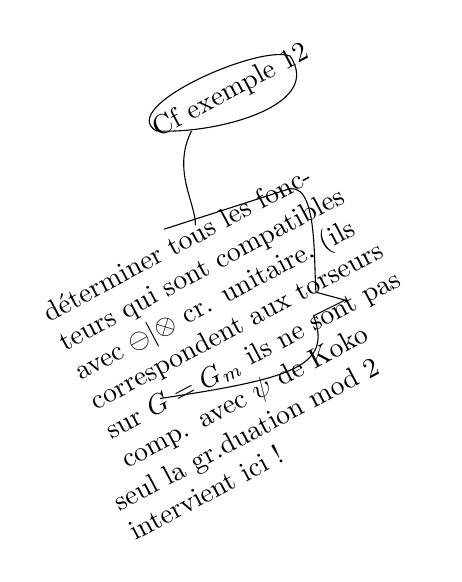
\begin{tikzpicture}[baseline]
\node[rotate=28] at (1.05,4.9) {\handwritten{Cf exemple 12}};
\draw (.1,4.4) .. controls (-.4,4.7) and (1.4,5.5) .. (1.8,5.35) .. controls (2.25,4.7) and (.8,4.35) .. (.1,4.4);
\draw (.55,4.4) .. controls (.3,3.9) and (.6,3.5) .. (.6,3.2);
\draw (.2,3.15)--(1.75,3.65) .. controls (2.15,3.8) and (2.1,2.8) .. (2.13,2.35)--(2.5,2.25)--(2.1,2.05) .. controls (2.35,1.4) and (1.8,1.25) .. (.15,1.0);
\node[rotate=28,align=left,text width=4.2cm] at (1.05,2.1) {\handwritten{déterminer tous les foncteurs qui sont compatibles avec $\unsure{\ominus|\otimes}$ cr. unitaire, \unsure{(}ils correspondent aux torseurs sur $G=G_m$ \uline{ils ne sont pas comp. avec $\psi$ \unsure{de} Koko}}};
\node[rotate=28,align=left,text width=3.9cm] at (1.4,.4) {\handwritten{seul la gr.duation mod $2$ intervient ici !}};
\end{tikzpicture}}}

8) Pour pallier à cet inconvénient, il y a lieu\deleted{lorsqu'on s'en va dans une catégorie avec $\otimes$ la catégorie des} d\deleted{e}'étudier systématiquement les $\otimes$-foncteurs compatib\rlap{e}l\rlap{s}es avec a)b)c) à valeurs dans une catégorie\inserted{de modules \unsure{grad|gradués}\handwritten{\begin{tikzpicture}[x=.48cm,y=.48cm,baseline=-.2ex]\draw (0,-.45) .. controls (-.08,.05) and (.16,.16) .. (.45,.17)--(2.7,.15) .. controls (2.93,.15) and (3.08,.19) .. (3.05,.4);\end{tikzpicture}}} $\unsure{\rlap{\(X\)}C|\mathbb{C}}$ comme ci-dessus: ce sont \rlap{d}\handwritten{l}es\handwritten{``}\uline{foncteurs fibres tordus}\handwritten{''}. En particulier, si $C$ est comme au début de 6) (pas encore de $\otimes$), supposons que le foncteur $F$ se factorise (de façon donnée) par les modules gradués, i.e. qu'on ait un foncteur compatible avec les foncteurs oublis $C\handwritten{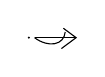
\begin{tikzpicture}[x=.6cm,y=.6cm,baseline=-.1ex]\fill (-.12,0) circle (.025);\draw (0,0)--(.85,0);\draw (0,0) .. controls (.3,-.22) and (.62,-.16) .. (.65,.12);\draw (.61,.2)--(.88,0)--(.57,-.23);\end{tikzpicture}}\mathrm{Gradf}(k)\unsure{\begin{tikzpicture}[x=1em,y=1em,baseline=-.1ex]\draw[line width=.6pt] (0,.32)--(.8,.32);\draw[line width=.8pt] (0,.08)--(.8,.08);\draw[line width=1.2pt] (.33,.08)--(.34,-.08);\draw[line width=.8pt] (.54,.08)--(.55,-.06);\end{tikzpicture}|=|\equiv}\mathbb{D}^{\unsure{\mathbb{X}|X}}$. Cela correspond à un homomorphisme de coalgèbres de $A$ dans $k\handwritten{[}T,T^{-1}\handwritten{]}$; où à la donnée d'éléments $\handwritten{\pi}_i$ de $U$ (les projections sur les composants homogènes) satisfaisant les conditions \deleted{$\unsure{\handwritten{\pi}}_i^2=0,\unsure{\handwritten{\pi}_i|i}$} habituelles
